
% --- Page 1: Cover / Section Break ---
\begin{center}
    \vspace*{\fill}
    % \fontsize{Size}{LineSpacing}\selectfont
    % Change 80 to 100 or 120 if you want it even bigger!
    \fontsize{28}{28}\selectfont \textbf{INTRODUCTION}
    \vspace*{\fill}
\end{center}
\clearpage
% --- Page 2: PHP Section ---
\vspace*{0.5cm}
\subheading{1. INTRODUCTION}
\vspace{0.5cm}
{ \normalfont \fontsize{12pt}{15pt}\selectfont
    \par
    \noindent Photography plays a crucial role in capturing and preserving memories at events such as weddings, convocations, college festivals, conferences, and cultural programmes. With the growing volume of digital photographs generated at these events, the development of an efficient and user-friendly system for organizing and distributing them has become essential. This project aims to design and implement SnapTrace, an online platform that uses facial recognition to deliver event photographs to the people who appear in them.\par
}
\vspace{0.4cm}
{ \normalfont \fontsize{12pt}{15pt}\selectfont
    \par
    \noindent The system is developed using React, Node.js, Express, and MySQL, with face-api, TensorFlow.js, and WebAssembly for facial-recognition processing, ensuring a responsive interface, reliable back-end processing, and secure data management. The primary objective is to provide a centralized platform where administrators, photographers, and attendees can interact seamlessly. Registered users upload a reference selfie, which is converted into a numerical facial descriptor. When event photographs are uploaded, the system detects faces, compares their descriptors with the stored ones, and adds the matching photographs to each user's personal gallery. \par
}
\vspace{0.4cm}

{ \normalfont \fontsize{12pt}{15pt}\selectfont
    \par
    \noindent The project also simplifies administrative operations by providing authentication, role-based access control, administrative functions, and audit logging within a single system. By integrating these features, SnapTrace reduces manual effort, speeds up photo distribution, and promotes controlled access and responsible handling of biometric information.
}
\vspace{0.4cm}

{ \normalfont \fontsize{12pt}{15pt}\selectfont
    \par
    \noindent Through this project, we demonstrate the practical application of web development, image processing, and database management concepts in addressing real-world challenges in event media management.
    \par
}
\vspace*{0.5cm}
\subheading{1.1 OBJECTIVES}
\vspace{0.5cm}
{ \normalfont \fontsize{12pt}{15pt}\selectfont
    \noindent The primary objectives of the SnapTrace: Intelligent Event Media Management and Biometric Distribution System are as follows: \par
}
\begin{itemize}
    \item \textbf{User-Friendly Platform:}
          \par \noindent To provide an intuitive and user-friendly web interface that enables attendees, photographers, and administrators to access and manage event media according to their respective roles.

    \item \textbf{Automated Photograph Identification:}
          \par \noindent To integrate facial-recognition technology that identifies faces in uploaded event photographs and compares them with registered users' facial descriptors to find potentially relevant images.

    \item \textbf{Efficient Event Media Management:}
          \par \noindent To streamline the process of uploading, processing, organizing, and distributing event photographs through an integrated web-based application, reducing the need for manual photograph searching.

    \item \textbf{Personalized Photo Galleries:}
          \par \noindent To provide registered users with galleries containing photographs associated with their accounts through the facial-matching process, making it easier to find relevant event memories.

    \item \textbf{Image Processing and Optimization:}
          \par \noindent To utilize image-processing techniques for validating, resizing, compressing, and generating thumbnails of photographs to support efficient media storage and presentation.

    \item \textbf{Secure User Authentication and Access Control:}
          \par \noindent To implement authentication and role-based authorization mechanisms that restrict access to protected application features according to the roles and permissions assigned to users.

    \item \textbf{Centralized Data Management:}
          \par \noindent To use a MySQL relational database for managing user accounts, settings, image metadata, gallery associations, administrative reports, audit records, and password-reset information.

    \item \textbf{Administrative Management and Monitoring:}
          \par \noindent To provide administrative functionality, reporting, and audit logging to support the management and monitoring of relevant activities within the application.

    \item \textbf{Asynchronous Image Processing:}
          \par \noindent To implement an in-process asynchronous queue that separates photograph-upload responses from subsequent facial-recognition and matching operations.

    \item \textbf{Privacy-Aware Media Distribution:}
          \par \noindent To consider privacy and controlled access when handling reference selfies, facial descriptors, and event photographs, while documenting the security and privacy limitations of the implemented system.

    \item \textbf{Future Scalability and Enhancement:}
          \par \noindent To establish a foundation for future improvements, including distributed job processing, cloud-based media storage, more efficient facial-descriptor searching, stronger authentication, and automated data-retention management.
\end{itemize}

\clearpage

\begin{center}
    \vspace*{\fill}
    % \fontsize{Size}{LineSpacing}\selectfont
    % Change 80 to 100 or 120 if you want it even bigger!
    \fontsize{28}{28}\selectfont \textbf{TECHNOLOGY PROFILE}
    \vspace*{\fill}
\end{center}
\clearpage

\vspace*{0.5cm}
{ \noindent \bfseries \fontsize{14pt}{15pt}\selectfont
    2. TECHNOLOGY PROFILE
    \par}
\vspace{0.4cm}

\par \noindent SnapTrace: Intelligent Event Media Management and Biometric Distribution System is developed using a combination of modern web technologies, backend frameworks, relational database systems, image-processing libraries, and computer-vision tools. These technologies work together to provide user authentication, event photograph uploads, facial recognition, image matching, gallery management, and administrative functionality. The selection of these technologies supports the integration of frontend development, backend processing, database operations, and biometric image analysis within a single web-based application.


\vspace{0.4cm}
{ \noindent \bfseries \fontsize{14pt}{15pt}\selectfont 1. React
}
\vspace{0.2cm}
\par \noindent React is a JavaScript library used to develop the user interface of SnapTrace. It enables the application to be divided into reusable components, making the interface easier to organize and maintain. React is used to build the frontend pages and interactive elements through which attendees, photographers, and administrators access the system's features.

\vspace{0.4cm}
{ \noindent \bfseries \fontsize{14pt}{15pt}\selectfont2. Vite
}
\vspace{0.2cm}
\par \noindent Vite is a frontend development and build tool used to run and build the React application. It provides a development server and a build process for preparing the frontend for deployment. In SnapTrace, Vite supports the development workflow and the delivery of the frontend application.

\vspace{0.4cm}
{ \noindent \bfseries \fontsize{14pt}{15pt}\selectfont3. React Router DOM
}
\vspace{0.2cm}
\par \noindent React Router DOM is used to manage navigation within the React application. It allows users to move between different application pages without requiring a complete browser-page reload for each navigation action. It supports the frontend routing structure of SnapTrace.

\vspace{0.4cm}
{ \noindent \bfseries \fontsize{14pt}{15pt}\selectfont4. HTML, CSS and JavaScript}

\vspace{0.2cm}
\par \noindent HTML provides the structural foundation of the web interface, while CSS controls its visual presentation and layout. JavaScript implements interactive behaviour and connects frontend components with backend API services. These technologies work together to create the user interface and support communication with the server.

\vspace{0.4cm}
{ \noindent \bfseries \fontsize{14pt}{15pt}\selectfont5. Node.js
    \par}

\vspace{0.2cm}
\par \noindent Node.js is a JavaScript runtime used to execute the SnapTrace backend. It provides the environment for running server-side application logic, processing API requests, coordinating image-processing tasks, and communicating with the database and computer-vision libraries.

\clearpage
\vspace*{0.5cm}
{ \noindent \bfseries \fontsize{14pt}{15pt}\selectfont6. Express.js
    \par}

\vspace{0.2cm}
\par \noindent Express.js is a web application framework for Node.js used to develop backend API endpoints. In SnapTrace, it manages HTTP requests and responses and connects application routes with controllers and supporting services. It also supports middleware-based authentication, authorization, and request processing.

\vspace{0.4cm}
{ \noindent \bfseries \fontsize{14pt}{15pt}\selectfont7. MySQL
    \par}

\vspace{0.2cm}
\par \noindent MySQL is a relational database management system used to store and manage the application's structured data. SnapTrace uses MySQL to maintain user accounts, user settings, image metadata, gallery associations, audit records, reports, and password-reset information. Relational constraints and database operations help maintain relationships between the records used by the application.

\vspace{0.4cm}
{ \noindent \bfseries \fontsize{14pt}{15pt}\selectfont8. Face-api
    \par}

\vspace{0.2cm}
\par \noindent Face-api is a JavaScript library used for face detection, facial-landmark processing, and facial-descriptor generation. In SnapTrace, it supports the computer-vision pipeline that detects faces in reference selfies and uploaded event photographs. The generated descriptors are used for facial comparison and the identification of potentially relevant photographs.

\vspace{0.4cm}
{ \noindent \bfseries \fontsize{14pt}{15pt}\selectfont9. TensorFlow.js
    \par}

\vspace{0.2cm}
\par \noindent TensorFlow.js provides machine-learning functionality in JavaScript environments. SnapTrace uses it as part of the backend computer-vision stack to execute the models required for facial processing. Its integration allows the application to perform the configured inference operations within the Node.js environment.

\vspace{0.4cm}
{ \noindent \bfseries \fontsize{14pt}{15pt}\selectfont10. WebAssembly (WASM)
    \par}

\vspace{0.2cm}
\par \noindent WebAssembly is a portable execution format that can run computational code in supported environments. SnapTrace uses the TensorFlow.js WebAssembly backend for computer-vision inference. This provides a machine-learning execution option within the JavaScript-based backend without requiring a separate GPU-based inference service.

\vspace{0.4cm}
{ \noindent \bfseries \fontsize{14pt}{15pt}\selectfont11. Sharp
    \par}

\vspace{0.2cm}
\par \noindent Sharp is an image-processing library used to prepare and manipulate image files. SnapTrace uses Sharp for image validation and processing operations, including resizing, compression, and thumbnail generation. These operations help prepare uploaded photographs for storage and presentation and support the processing of reference selfies.
\clearpage
\vspace*{0.5cm}
{ \noindent \bfseries \fontsize{14pt}{15pt}\selectfont12. Multer
    \par}
\vspace{0.2cm}
\par \noindent Multer is middleware for handling multipart form-data requests, particularly file uploads, in Node.js and Express applications. In SnapTrace, it supports the reception of uploaded reference selfies and event photographs through the backend. Additional validation is used to enforce the application's supported file types and upload-size limits.

\vspace{0.4cm}
{ \noindent \bfseries \fontsize{14pt}{15pt}\selectfont13. JSON Web Token (JWT)
    \par}

\vspace{0.2cm}
\par \noindent JSON Web Token is a token-based mechanism used to represent authentication information between the client and server. SnapTrace uses JWT-based authentication to identify authenticated users when accessing protected backend endpoints. The application also implements token invalidation support for relevant account-security changes.

\vspace{0.4cm}
{ \noindent \bfseries \fontsize{14pt}{15pt}\selectfont14. Bcrypt
    \par}

\vspace{0.2cm}
\par \noindent Bcrypt is a password-hashing library used to protect user passwords. Instead of storing passwords as ordinary readable text, the application stores password hashes that can be verified during authentication. SnapTrace uses this mechanism as part of its account-security implementation.

\vspace{0.4cm}
{ \noindent \bfseries \fontsize{14pt}{15pt}\selectfont15. Vitest
    \par}
\vspace{0.2cm}
\par \noindent Vitest is a JavaScript and TypeScript testing framework used for automated backend tests in SnapTrace. The documented test baseline contains five backend test suites with 44 passing tests. These tests verify selected application behaviour, but they do not establish complete frontend, end-to-end, or biometric-accuracy test coverage.

\vspace{0.4cm}
{ \noindent \bfseries \fontsize{14pt}{15pt}\selectfont16. In-Process Asynchronous Queue
    \par}
\vspace{0.2cm}
\par \noindent SnapTrace uses an in-process JavaScript queue to schedule facial-matching tasks after event photographs are uploaded. This approach allows the upload response to be returned before all matching operations are completed. The queue uses a single worker and is stored in application memory; it is not a distributed or durable job-processing system.
\clearpage

\begin{center}
    \vspace*{\fill}
    % \fontsize{Size}{LineSpacing}\selectfont
    % Change 80 to 100 or 120 if you want it even bigger!
    \fontsize{28}{28}\selectfont \textbf{SYSTEM STUDY}
    \vspace*{\fill}
\end{center}
\clearpage


\vspace*{0.5cm}
{ \noindent \bfseries \fontsize{14pt}{15pt}\selectfont
    3. SYSTEM STUDY
    \par}
\vspace{0.4cm}

\para{System study is an important phase in the development of any software system. It involves examining the existing methods, identifying their limitations, understanding user requirements, and evaluating possible solutions to determine the most suitable approach. In SnapTrace, the system study focuses on the challenges involved in managing and distributing digital photographs generated during events such as college festivals, convocations, conferences, weddings, and other social or professional gatherings. The study examines the difficulties associated with manually identifying photographs, organizing large image collections, and distributing relevant photographs to individual participants. Based on these observations, an automated, web-based solution using facial-recognition technology is proposed. The system study also considers the functional requirements, user roles, database management, image-processing workflow, access control, and privacy considerations necessary for developing an effective event media management system.}
\heading{3.1 EXISTING SYSTEM}
\para{The existing methods of event photograph management commonly depend on manual organization and conventional photo-sharing platforms. After an event, photographers and event organizers generally upload photographs to shared folders, online albums, websites, or cloud storage platforms. Participants must browse through these collections to find photographs in which they appear. When an event contains hundreds or thousands of photographs, locating a particular individual's images can become a time-consuming and inconvenient process.
    Manual identification also increases the workload of photographers and event organizers, who may need to sort photographs, create separate collections, or respond to individual requests. Traditional photo-sharing methods generally organize images by folders, filenames, or event categories rather than automatically identifying the people appearing in them. As a result, users may need to examine numerous photographs before finding the images relevant to them. Another limitation is the difficulty of distributing photographs to the appropriate individuals in an organized manner. Sharing a common folder provides convenient access to a large collection, but it does not automatically create personalized galleries for individual participants. It can also be difficult to manage access to photographs when several users, photographers, and administrators are involved.
    Conventional workflows may also provide limited integration between facial identification, image processing, user authentication, and administrative monitoring. Without an automated identification mechanism, organizing and retrieving relevant photographs becomes increasingly difficult as the size of an event's image collection grows.
    These limitations highlight the need for an intelligent event media management system that can automate photograph identification, associate relevant images with registered users, and provide personalized galleries through a web-based application.
}
\clearpage
\heading{3.2 PROPOSED SYSTEM}
\para{
    The proposed \textbf{SnapTrace — Intelligent Event Media Management \& Biometric Distribution System} aims to overcome the limitations of conventional photo-sharing methods by integrating facial-recognition technology with web-based image management. The system provides a platform through which users can register, submit a reference selfie, and access event photographs identified as potentially matching their facial features.
    \vspace{0.4cm}
    \noindent SnapTrace is developed using \textbf{React} for the frontend, \textbf{Node.js and Express.js} for backend services, and \textbf{MySQL} for data storage. The facial-recognition pipeline uses \textbf{@vladmandic/face-api}, TensorFlow.js, and the WebAssembly backend to detect faces, extract facial landmarks, generate numerical facial descriptors, and compare these descriptors with registered users' descriptors. The Sharp image-processing library is used to resize and optimize uploaded images and generate thumbnails.
    \vspace{0.4cm}
    \noindent When a user submits a reference selfie, the system validates and processes the image and generates a 128-dimensional facial descriptor. When photographers upload event photographs, the system stores and processes the images and performs face matching in the background. Photographs identified as matching a registered user's facial descriptor can then be associated with that user and displayed in the user's personalized gallery.
    \vspace{0.4cm}
    \noindent The system includes separate access and functionality for users, photographers, and administrators. Authentication and role-based authorization help restrict access to relevant operations. Administrative functions support system management and monitoring, while audit logging records selected administrative activities. The backend uses an asynchronous in-process queue to process uploaded photographs without requiring the upload request to wait for the entire matching operation to finish.
    \vspace{0.4cm}
    \noindent SnapTrace aims to reduce the manual effort involved in identifying and distributing event photographs, improve image retrieval, and provide a more organized user experience. However, facial matches are based on a configured similarity threshold and should be understood as automated matching results rather than a guarantee of perfect identification. The system also requires responsible handling of selfies, facial descriptors, and event photographs, with appropriate attention to privacy and access control.

}
\clearpage
\heading{3.3 MODULE DESCRIPTION}

\para{SnapTrace is divided into functional modules that work together to support user registration, event photograph processing, facial matching, personalized gallery management, and administration.
}
\subheading{1. User Module}

Functionalities of User:
\begin{itemize}
    \item \textbf{User Registration: } \noindent Allows new users to create accounts by providing necessary information and a reference selfie.
    \item \textbf{Login: } \noindent Authenticate themselves to access the application.
    \item \textbf{Password Reset: } \noindent Provides a password recovery mechanism through a reset link.
    \item \textbf{Profile Management: } \noindent Supports access to and management of available user profile information.
    \item \textbf{Selfie Enrollment: } \noindent Allows users to upload a reference selfie for facial-descriptor generation.
    \item \textbf{Personalized Photo Gallery: } \noindent Enables users to view event photographs associated with their accounts through the face-matching process.
    \item \textbf{Gallery Management: } \noindent Supports access to matched photographs and related gallery information.
    \item \textbf{User Settings: } \noindent Allows users to access and update supported application preferences.
\end{itemize}

\subheading{2. Photographer Module}

Functionalities of Photographer:

\begin{itemize}
    \item \textbf{Login and Authentication: } \noindent Provides authenticated access to photographer-related functionality.
    \item \textbf{Event Photograph Upload: } \noindent Allows photographers to upload event photographs in supported image formats.
    \item \textbf{Image Validation: } \noindent Validates uploaded files against supported formats and configured file-size and upload-count limits.
    \item \textbf{Background Face Matching: } \noindent Initiates asynchronous processing to detect faces and compare facial descriptors.
    \item \textbf{Photo Distribution: } \noindent Supports associating matched photographs with the relevant registered users.
    \item \textbf{Upload Status and Results: } \noindent Provides access to available information about uploaded images and their processing results.
\end{itemize}

\subheading{3. Administrator Module}

Functionalities of Admin:

\begin{itemize}
    \item \textbf{Administrative Authentication: } \noindent Provides access to administrative operations for authorized users.
    \item \textbf{User Management: } \noindent Supports viewing and managing user information through available administrative functionality.
    \item \textbf{Photographer Management: } \noindent Supports relevant account and system-management operations for photographers.
    \item \textbf{System Monitoring: } \noindent Provides access to available administrative information about the application's operation.
    \item \textbf{Audit Log Management: } \noindent Records and supports the review of selected administrative activities.
    \item \textbf{Report Management: } \noindent Supports the generation and management of reports in the implemented reporting workflow.
    \item \textbf{Access Control: } \noindent Uses role-based authorization to restrict administrative operations to permitted users.
\end{itemize}

\subheading{4. Facial Recognition and Image Processing Module}

Functionalities of the Module:
\begin{itemize}
    \item \textbf{Face Detection: } \noindent Detects faces in uploaded selfies and event photographs using the configured face-detection model.
    \item \textbf{Facial Landmark Detection: } \noindent Identifies facial landmarks to support the facial-recognition pipeline.
    \item \textbf{Facial Descriptor Generation: } \noindent Generates a 128-dimensional numerical descriptor representing detected facial features.
    \item \textbf{Descriptor Comparison: } \noindent Compares facial descriptors using Euclidean distance.
    \item \textbf{Match Decision: } \noindent Uses a configured distance threshold of 0.50 or lower to identify potential matches.
    \item \textbf{Image Optimization: } \noindent Resizes uploaded images and generates thumbnails to support efficient storage and display.
    \item \textbf{Asynchronous Processing: } \noindent Processes event photographs through an in-process background queue.
\end{itemize}

\subheading{5. Database and Data Management Module}

Functionalities of the Module:
\begin{itemize}
    \item \textbf{User Data Management: } \noindent Stores and retrieves registered user information.
    \item \textbf{Facial Descriptor Storage: } \noindent Stores facial descriptors in the database for subsequent comparison.
    \item \textbf{Photograph Metadata Management: } \noindent Maintains image records and associated metadata.
    \item \textbf{Personalized Gallery Mapping: } \noindent Maintains associations between users and photographs identified as matches.
    \item \textbf{Settings Management: } \noindent Stores user settings when they are explicitly created or updated.
    \item \textbf{Report Metadata Management: } \noindent Maintains report-related records in the database.
    \item \textbf{Password Reset Records: } \noindent Maintains password-reset tokens and their associated expiry and usage information.
\end{itemize}

\subheading{6. Authentication and Security Module}

Functionalities of the Module:
\begin{itemize}

    \item \textbf{Password Protection: } \noindent Uses password hashing to protect stored account passwords.
    \item \textbf{Token-Based Authentication: } \noindent Uses JSON Web Tokens (JWT) to authenticate users.
    \item \textbf{Role-Based Authorization: } \noindent Restricts protected operations according to the user's role.
    \item \textbf{Signed Media URLs: } \noindent Supports time-limited, HMAC-SHA256-signed URLs for controlled media access.
    \item \textbf{Input Validation: } \noindent Validates supported upload formats and configured file restrictions.
    \item \textbf{Administrative Auditing: } \noindent Records selected administrative actions to support accountability.
\end{itemize}

\clearpage


\begin{center}
    \vspace*{\fill}
    % \fontsize{Size}{LineSpacing}\selectfont
    % Change 80 to 100 or 120 if you want it even bigger!
    \fontsize{28}{28}\selectfont \textbf{SYSTEM ANALYSIS}
    \vspace*{\fill}
\end{center}
\clearpage

\heading{4. SYSTEM ANALYSIS}

\subheading{4.1 INTRODUCTION}

\para{System analysis is an important phase in the software development process. It involves identifying the problems associated with the existing system, understanding user requirements, examining the operations to be performed, and determining a suitable solution. In the development of SnapTrace, system analysis focuses on the difficulties involved in manually organizing, identifying, and distributing event photographs. The analysis examines how facial-recognition technology can be integrated with a web-based application to simplify photograph identification and provide personalized galleries for registered users. It also considers the requirements for user authentication, image processing, database management, administrative operations, and controlled access to photographs. Based on this analysis, SnapTrace is designed to provide an automated and organized approach to event media management using modern web technologies.}

\subheading{4.2 DEFINITION}

\para{System analysis is the systematic study of a proposed or existing system to understand its components, functions, operations, and relationships. It involves breaking down the system into smaller functional units to identify requirements, limitations, and possible improvements. In SnapTrace, system analysis examines the interaction between the frontend, backend services, database, facial-recognition pipeline, and different user roles to determine how the application can efficiently identify and distribute relevant event photographs.}

\subheading{4.3 OBJECTIVES}

\para{The main objectives of system analysis for SnapTrace are as follows:}
\begin{itemize}
    \item \textbf{Understanding the Existing System:} To study conventional methods of event photograph storage and sharing and identify the difficulties associated with manually finding relevant photographs.
    \item \textbf{Identifying System Requirements:} To determine the functional and technical requirements needed for user registration, selfie enrollment, photograph uploads, facial matching, and personalized gallery management.
    \item \textbf{Developing the Proposed System:} To design a web-based event media management system that uses facial-recognition technology to automate the identification of potentially relevant photographs.
    \item \textbf{Efficient Image Processing:} To analyze and implement the processes required to detect faces, generate facial descriptors, compare them, and associate matching photographs with registered users.
    \item \textbf{Database Management:} To organize user information, facial descriptors, photograph metadata, gallery associations, and other application records using a relational database.
    \item \textbf{User-Friendly Interface:} To provide an accessible and organized interface through which users, photographers, and administrators can perform their respective operations.
    \item \textbf{Authentication and Access Control:} To incorporate authentication and role-based authorization to restrict access to protected application features.
    \item \textbf{Reducing Manual Effort:} To minimize the time and effort required to identify and distribute photographs compared with conventional manual methods.
    \item \textbf{Privacy and Data Protection:} To consider appropriate handling of selfies, facial descriptors, and event photographs, including access restrictions and responsible data management.
    \item \textbf{System Reliability and Maintainability:} To organize the application into functional components that can be tested, maintained, and improved as requirements evolve.
\end{itemize}

\clearpage
\begin{center}
    \vspace*{\fill}
    % \fontsize{Size}{LineSpacing}\selectfont
    % Change 80 to 100 or 120 if you want it even bigger!
    \fontsize{28}{28}\selectfont \textbf{SYSTEM SPECIFICATION}
    \vspace*{\fill}
\end{center}

\clearpage
\heading{5. SYSTEM SPECIFICATION}

\subheading{5.1 SOFTWARE SPECIFICATIONS}

\para{A Software Requirements Specification (SRS) describes the functional and non-functional requirements of a software system. It provides a detailed overview of the system's expected behaviour, software components, operating environment, and implementation constraints. It helps ensure that the developed application meets the intended requirements and provides a clear understanding of the technologies required for development and execution.}

\para{SnapTrace is a web-based Intelligent Event Media Management and Biometric Distribution System developed to automate the identification and distribution of event photographs using facial-recognition technology. The software environment consists of frontend technologies for the user interface, backend technologies for application logic, a relational database for data storage, and computer-vision libraries for facial recognition and image processing.}

The software requirements for SnapTrace are as follows:
\begin{itemize}
    \item \textbf{Operating System:} Windows 10 or Windows 11, or a compatible Linux operating system.
    \item \textbf{Frontend:} React 19, Vite 8, React Router DOM 7, HTML, CSS, and JavaScript.
    \item \textbf{Backend:} Node.js 20 or above and Express.js 4.21.2.
    \item \textbf{Database:} MySQL Community Server 8.0.46.
    \item \textbf{Database Connectivity:} MySQL2 with Promise-based support.
    \item \textbf{Facial Recognition:} @vladmandic/face-api 1.7.15.
    \item \textbf{Machine Learning Framework:} TensorFlow.js with the WebAssembly backend.
    \item \textbf{Image Processing:} Sharp for image resizing, optimization, and thumbnail generation.
    \item \textbf{Authentication and Security:} JSON Web Tokens (JWT) and Bcrypt.
    \item \textbf{File Upload Management:} Multer.
    \item \textbf{Email Service:} Nodemailer for password-reset email functionality.
    \item \textbf{Testing Framework:} Vitest for backend testing.
    \item \textbf{Web Browser:} Google Chrome, Mozilla Firefox, Microsoft Edge, or another modern browser compatible with the application's frontend.
    \item \textbf{Development Tools:} Visual Studio Code or another suitable code editor, Node.js package management tools, and MySQL administration tools.
\end{itemize}
These technologies work together to provide a web-based platform for user authentication, selfie enrollment, event photograph uploads, facial matching, personalized galleries, and administrative operations. The React frontend communicates with the Express backend through API endpoints, while MySQL stores user information, image metadata, facial descriptors, gallery associations, and other application records.

\subheading{5.2 HARDWARE SPECIFICATION}

\para{Hardware specifications describe the physical resources required to develop, execute, and test a software application. The required configuration depends on the size of the image collection, the number of users, and the computational workload involved in facial-recognition processing.}

\para{SnapTrace performs image processing and facial matching on the backend. Therefore, adequate processor performance, memory, and storage capacity are important for handling uploaded photographs and processing facial descriptors. The following configuration provides a practical guideline for development and testing.}
\vspace{0.4cm}
\noindent \textbf{Minimum Hardware Requirements}
\begin{itemize}
    \item \textbf{Processor:} Dual-core processor or equivalent.
    \item \textbf{Memory (RAM):} 4 GB.
    \item \textbf{Storage:} At least 10 GB of available disk space for the application, dependencies, database, and test images.
    \item \textbf{Display:} Standard PC monitor or laptop display.
    \item \textbf{Input Devices:} Keyboard and mouse or compatible touchpad.
    \item \textbf{Network:} Internet or local network connectivity for communication between the frontend, backend, and database when deployed separately.
\end{itemize}

\vspace{0.4cm}
\noindent \textbf{Recommended Hardware Requirements}

\begin{itemize}
    \item \textbf{Processor:} Quad-core Intel or AMD processor or equivalent.
    \item \textbf{Memory (RAM):} 8 GB to 16 GB.
    \item \textbf{Storage:} SSD with sufficient free space for application files, database records, uploaded photographs, thumbnails, and reports.
    \item \textbf{Display:} Standard HD display or higher.
    \item \textbf{Input Devices:} Keyboard and mouse or compatible touchpad.
    \item \textbf{Network:} Stable broadband or local network connection.

\end{itemize}
\heading{6. FEASIBILITY ANALYSIS}

\para{The feasibility analysis for \textbf{SnapTrace — Intelligent Event Media Management \& Biometric Distribution System} evaluates the practicality of developing and implementing the project in terms of technical, economic, operational, schedule, and legal feasibility. This analysis helps determine whether the proposed system can be developed using the available technologies, resources, and time while meeting its intended objectives. SnapTrace aims to simplify event photograph management by using facial-recognition technology to identify potentially relevant photographs and associate them with registered users. The feasibility study examines the suitability of the technology stack, development costs, usability, project schedule, and considerations related to the handling of personal and biometric information.}
\subheading{6.1 TECHNICAL FEASIBILITY}

\para{SnapTrace is technically feasible because it uses established web development technologies and machine-learning libraries. The frontend is developed using React, while Node.js and Express.js provide backend services. MySQL is used for structured data storage, and @vladmandic/face-api, TensorFlow.js, and the WebAssembly backend support facial detection and descriptor comparison. The Sharp library is used for image resizing, optimization, and thumbnail generation.
    These technologies support the implementation of user registration, authentication, selfie enrollment, event photograph uploads, facial matching, and personalized photo galleries. The system uses a modular architecture that separates the frontend, backend, database, and image-processing operations. This organization supports testing and maintenance.
    However, facial-recognition performance depends on factors such as image quality, lighting, face orientation, and the number of photographs being processed. The current system uses an in-process asynchronous queue rather than a distributed job-processing service. Therefore, the implementation is suitable for its intended development and small-to-medium event use cases, while larger deployments may require additional infrastructure and performance evaluation.}

\subheading{6.2 ECONOMIC FEASIBILITY}

\para{SnapTrace is economically feasible because its principal development technologies are available as open-source software or through freely available development tools. React, Node.js, Express.js, MySQL Community Server, and the facial-recognition libraries help reduce software licensing costs. The application can be developed and tested on an existing computer without requiring dedicated commercial machine-learning hardware.
    The main costs associated with the project may include computer hardware, internet connectivity, database and media storage, deployment infrastructure, domain registration, and maintenance. Additional expenses may arise if the system is deployed on a paid hosting platform or requires increased storage and processing capacity.
    Since the project uses existing software libraries and a web-based architecture, the initial development cost can be kept relatively low. The expected benefits include reduced manual effort in locating photographs, more organized image distribution, and improved convenience for event participants. Actual cost savings will depend on the scale of deployment and the resources required to operate the system.
}
\subheading{6.3 OPERATIONAL FEASIBILITY}

\para{SnapTrace is operationally feasible because it provides separate functionality for registered users, photographers, and administrators. Users can register, submit a reference selfie, and view photographs associated with their accounts. Photographers can upload event photographs for processing, while administrators can access the available management, reporting, and audit-related functions.
    The web-based interface allows users to access the system through a compatible browser without requiring a separate desktop application. Automated face detection and descriptor comparison reduce the need to manually inspect every photograph to identify potential matches. Background processing also allows the upload request to finish before the complete matching workflow has finished.
    The system nevertheless requires users to provide suitable reference selfies and photographers to upload supported image files. Facial matching results may not always be accurate, so the system should not be treated as guaranteeing correct identification. Appropriate access controls and responsible handling of selfies, facial descriptors, and event photographs are also necessary for practical use.
}
\subheading{6.4 SCHEDULE FEASIBILITY}

\para{SnapTrace is schedule-feasible when developed through a structured, incremental approach. The project can be divided into stages such as requirement analysis, frontend development, backend and database implementation, facial-recognition integration, image-processing implementation, and testing.
    The modular structure allows individual components to be developed and verified before they are integrated into the complete application. Existing frameworks and libraries also reduce the need to implement common functions, such as routing, database connectivity, authentication, and image processing, entirely from scratch.
    The project includes backend unit tests to verify selected application functions. However, the facial-recognition workflow and background-processing queue are not comprehensively covered by those unit tests, and frontend end-to-end testing has not been established. Additional integration and performance testing would therefore be required before a larger production deployment. The overall schedule feasibility depends on the project deadline, available development time, and the effort needed for verification and refinement.
}
\clearpage
\subheading{6.5 LEGAL FEASIBILITY}
\para{
    SnapTrace processes personal information, including account details, reference selfies, facial descriptors, and event photographs. Therefore, privacy, security, and responsible data handling are important considerations in its development and deployment.
}
\para{The system incorporates certain protective measures, including password hashing, token-based authentication, role-based authorization, and controlled media-access mechanisms. These features help reduce the risk of unauthorized access to protected application functions. The system also supports account-related data management and records selected administrative activities.}

\para{However, the presence of these technical controls does not establish legal compliance or certification. The implementation has limitations that require attention, including the need for stronger controls over direct access to uploaded media, a secure and consistent configuration of signing secrets, and a defined data-retention and deletion process. Clear user consent, appropriate privacy notices, and procedures for handling personal data should also be addressed before deployment.}

\para{The project should be evaluated against applicable Indian data-protection requirements, including the Digital Personal Data Protection Act, 2023, and relevant rules and commencement provisions applicable at the time of deployment. Consequently, SnapTrace is technically designed with certain privacy and security considerations, but its legal compliance must be assessed separately before it is used in a real-world environment.
}
\clearpage

\begin{center}
    \vspace*{\fill}
    % \fontsize{Size}{LineSpacing}\selectfont
    % Change 80 to 100 or 120 if you want it even bigger!
    \fontsize{28}{28}\selectfont \textbf{SYSTEM DESIGN}
    \vspace*{\fill}
\end{center}
\clearpage


\heading{7. SYSTEM DESIGN}

\para{System design is an important phase in software development that translates the requirements identified during system analysis into a structured software solution. It defines the architecture, components, data flow, input and output processes, database structure, and interactions between different parts of the application. The purpose of system design is to establish a clear plan for implementing a system that meets the specified requirements while remaining maintainable and reliable.}

\para{In SnapTrace, the system design focuses on developing an intelligent event media management and biometric distribution system that automates the identification and distribution of event photographs. The design integrates a React-based frontend, a Node.js and Express backend, a MySQL database, and a facial-recognition pipeline. It defines how users register and submit reference selfies, how photographers upload event photographs, how facial descriptors are generated and compared, and how matched photographs are associated with individual user galleries.}

\para{The design is divided into logical and physical aspects. Logical design describes the major components, their relationships, the information flowing through the system, and the data stored in the database. Physical design describes the implementation using the selected programming languages, frameworks, libraries, database tables, and application services.}

\heading{7.1 ARCHITECTURAL DESIGN}

\para{Software architectural design defines the major components of a system and the relationships between them. It provides a structural framework for understanding how the application operates and how its components communicate with one another.}

\para{SnapTrace follows a \textbf{three-tier web application architecture} consisting of the presentation layer, application layer, and data layer.}

\subheading{7.1.1. Presentation Layer}

\para{The presentation layer is developed using React 19, Vite 8, React Router DOM 7, HTML, CSS, and JavaScript. It provides the user interface through which users, photographers, and administrators interact with the application. It supports account-related operations, selfie submission, photograph uploads, gallery access, and administrative functions.}

\subheading{7.1.2. Application Layer}

\para{The application layer is implemented using Node.js and Express.js. It handles API requests, authentication, role-based authorization, input validation, file uploads, image-processing operations, facial recognition, and database communication. The application uses an asynchronous in-process queue to process uploaded photographs in the background.}
\clearpage
\subheading{7.1.3. Data Layer}

\para{The data layer uses MySQL Community Server to store structured application information. The database maintains user records, user settings, image metadata, user-gallery associations, administrative audit records, reports, and password-reset tokens. Facial descriptors are stored as JSON data associated with user records. The facial-recognition pipeline operates within the backend processing workflow. It uses @vladmandic/face-api, TensorFlow.js, and the WebAssembly backend to detect faces, identify facial landmarks, generate 128-dimensional facial descriptors, and compare descriptors using Euclidean distance.}

\para{The overall architecture can be represented as:}

\para{\textbf{User / Photographer / Administrator $\rightarrow$ React Frontend $\rightarrow$ Express REST API $\rightarrow$ Application Services $\rightarrow$ MySQL Database}}

\para{The facial-recognition and image-processing services are invoked by the backend as required. Uploaded photographs are processed asynchronously, and potential matches are associated with the relevant users.}

\heading{7.2 INPUT DESIGN}

\para{Input design specifies how information enters the system, how it is validated, and how it is processed. A well-designed input mechanism helps reduce invalid data, prevents avoidable processing errors, and provides users with a consistent interaction experience.}

\para{In SnapTrace, input design covers account information, reference selfies, event photographs, user settings, and administrative requests. The application validates inputs before performing the corresponding operations.}

\para{The major inputs are described below.}

\subheading{1. User Registration Input}

\para{Users provide the information required to create an account. The backend validates the submitted data before storing the account information in the database. Passwords are hashed using Bcrypt before storage.}

\subheading{2. Login Input}

\para{Users submit their login credentials through the authentication interface. The backend verifies the credentials and issues a JSON Web Token (JWT) when authentication succeeds. Protected operations require appropriate authentication and authorization.}

\subheading{3. Reference Selfie Input}

\para{A registered user can upload a reference selfie for facial enrollment. The accepted image formats are JPEG and PNG, with a maximum file size of 5 MB. The image is processed using Sharp, with its maximum dimension reduced to 600 pixels. The facial-recognition pipeline requires exactly one detected face for enrollment. A 128-dimensional facial descriptor is generated and stored in the database.}

\subheading{4. Event Photograph Input}

\para{Photographers can upload event photographs for processing. The system accepts JPEG and PNG images, with a maximum size of 30 MB per file and a maximum of 10 files per request. Sharp is used to resize and optimize the images and generate thumbnails.}

\subheading{5. User Settings Input}

\para{Users can update the application preferences supported by the system. The backend validates and stores the settings in the database when they are explicitly created or updated.}

\subheading{6. Administrative Input}

\para{Authorized administrators submit requests for available administrative functions, including user management, report-related operations, and other supported management activities. Role-based authorization restricts access to protected operations.}

\para{Input validation and appropriate error responses help prevent unsupported file formats, oversized uploads, invalid authentication requests, and other avoidable processing problems.}

\heading{7.3 OUTPUT DESIGN}

\para{Output design describes how processed information is presented to users. The output should be clear, organized, and relevant to the user's role and activities. SnapTrace provides application outputs through its web interface and supporting API responses.}

\para{The main outputs of the system include the following:}

\subheading{1. Authentication Output}

\para{The system provides authentication results and appropriate responses for successful or unsuccessful login and password-reset operations.}

\subheading{2. Personalized Photo Gallery}

\para{Users can view photographs associated with their accounts through the personalized gallery. These associations are generated through the facial-matching workflow.}

\subheading{3. Photograph Upload Response}

\para{After uploaded files have been accepted and stored, the backend returns an HTTP 201 response before background facial matching is necessarily complete. Therefore, successful upload acceptance does not mean that every photograph has already been processed or matched.}
\clearpage
\subheading{4. Facial-Matching Output}

\para{The matching process compares facial descriptors using Euclidean distance. A distance of 0.50 or lower is treated as a potential match according to the configured threshold. The matching workflow produces associations between photographs and registered users when the configured criteria are satisfied.}

\subheading{5. Image and Thumbnail Output}

\para{The system generates optimized image files and thumbnails to support image display and retrieval.}

\subheading{6. Administrative Output}

\para{Authorized administrators can access available management information, selected audit records, and report-related outputs.}

\subheading{7. Report Output}

\para{The reporting workflow generates JSON report files in the backend uploads directory and maintains associated metadata in the database.}

\para{The output design aims to provide an organized way to access photographs and administrative information. The accuracy of facial matching depends on image quality and other factors, so matching results should not be interpreted as a guarantee of correct identification.}
\clearpage
\heading{7.4 DATABASE DESIGN}

\para{Database design defines how information is organized, stored, related, and retrieved. SnapTrace uses MySQL Community Server with the InnoDB storage engine and the utf8mb4\_unicode\_ci character collation. The database supports the storage and management of account information, facial descriptors, image records, gallery associations, and administrative data.}

\para{The database consists of seven live physical tables.}

\subheading{1. users}

\para{This table stores registered user information and account-related data. It also contains the face\_embedding field, which stores the user's 128-dimensional facial descriptor as JSON data. The user's updated\_at field reflects updates to the user record.}

\subheading{2. user\_settings}

\para{This table stores user preferences when a settings record has been explicitly created or updated. The application can return default settings when no corresponding record exists.}

\subheading{3. images}

\para{This table stores image-related information and metadata required by the application for managing uploaded photographs.}

\subheading{4. user\_gallery\_photos}

\para{This table maintains the association between users and photographs identified as potential matches. It supports a many-to-many relationship between users and images and stores match-related information, including confidence values. A unique constraint on (user\_id, photo\_id) prevents duplicate associations for the same user and photograph.}

\subheading{5. admin\_audit\_log}

\para{This table records selected administrative activities to support accountability and operational review.}

\subheading{6. reports}

\para{This table stores metadata associated with generated reports. The corresponding report contents are written to JSON files.}
\clearpage
\subheading{7. password\_reset\_tokens}

\para{This table stores password-reset token records, including information related to token usage and expiry.}

\subheading{Primary Key:} \para{A primary key uniquely identifies a record in a table. It helps maintain the identity of individual database records.}

\subheading{Foreign Key:} \para{A foreign key establishes a relationship between records in different tables and helps maintain referential integrity. SnapTrace uses relational associations to connect users, images, and gallery records.}

\subheading{Normalization:} \para{Database normalization organizes data to reduce unnecessary duplication and improve consistency. SnapTrace uses relational tables and defined relationships to structure its application data. The database design should be evaluated against normalization principles and the specific constraints of each table.}

\subheading{Database Relationships}

\para{The main database relationships include:}

\begin{itemize}
    \item User records are associated with user settings where a settings record exists.
    \item User records are associated with facial descriptors used during matching.
    \item Image records are associated with users through the user\_gallery\_photos mapping table.
    \item Report records maintain metadata for generated report files.
    \item Password-reset records are associated with accounts and their reset operations.
\end{itemize}

\para{The user\_gallery\_photos table is present in the live database and schema dump. However, the available migration files do not fully reproduce the live schema, so the migration set requires correction before it can be relied upon to recreate the complete database independently.}

\clearpage
\heading{7.5 MODULARIZATION}

\para{Modularization is the process of dividing a software system into smaller functional units. Each module is responsible for a specific group of related operations. This approach improves code organization, simplifies testing, and makes maintenance easier because changes can often be made within a particular component without affecting the entire application.}

\para{SnapTrace is organized into the following functional modules:}

\begin{itemize}
    \item \textbf{Authentication Module:} Handles account authentication, JWT generation and validation, password hashing, and password-reset operations.
    \item \textbf{User Management Module:} Handles user records, profile-related operations, and supported user settings.
    \item \textbf{Selfie Enrollment Module:} Accepts reference selfies, validates uploaded files, and generates facial descriptors.
    \item \textbf{Photograph Upload Module:} Accepts event photographs, validates files, and stores the uploaded images.
    \item \textbf{Image Processing Module:} Resizes images, optimizes image files, and generates thumbnails using Sharp.
    \item \textbf{Facial Recognition Module:} Detects faces, identifies facial landmarks, generates descriptors, and compares facial descriptors.
    \item \textbf{Gallery Management Module:} Maintains associations between users and photographs identified as potential matches.
    \item \textbf{Administrative Module:} Supports available administrative functions and records selected administrative activities.
    \item \textbf{Reporting Module:} Generates JSON reports and maintains their metadata.
    \item \textbf{Database Access Module:} Provides database operations for retrieving and modifying application data.
\end{itemize}

\para{The modules communicate through defined application interfaces and backend services. This structure makes the application easier to understand and provides a basis for future improvements.}
\clearpage
\heading{7.6 CODING PHASE}

\para{The coding phase translates the system design into executable software. During this phase, the frontend, backend, database operations, authentication mechanisms, and facial-recognition functionality are implemented using the selected technologies.}

\para{The SnapTrace frontend is developed using React and JavaScript, with Vite supporting the development and build process. React Router DOM manages frontend navigation. The interface communicates with the backend through REST API endpoints.}

\para{The backend uses Node.js and Express.js to implement API routes, request handling, authentication, authorization, file uploads, and application logic. The mysql2/promise library provides Promise-based database connectivity. Bcrypt is used for password hashing, and JWT is used for token-based authentication.}

\para{The facial-recognition workflow uses @vladmandic/face-api and TensorFlow.js with the WebAssembly backend. Sharp performs image-processing operations, while Multer manages multipart file uploads. An in-process asynchronous queue coordinates background processing of event photographs.}

\para{The coding process also includes input validation, error handling, database operations, and testing of implemented functions. The backend is tested using Vitest. The existing automated tests verify selected backend behaviour, but comprehensive browser end-to-end testing and full evaluation of facial-recognition accuracy remain outside the demonstrated test coverage.}

\heading{7.7 CODING DESIGN}

\para{Coding design establishes conventions that improve readability, reliability, and maintainability. A well-organized codebase uses meaningful names, separates responsibilities, validates inputs, and handles errors consistently.}

\para{SnapTrace uses a component-based frontend structure and a backend organized around API routes and application logic. The frontend components are responsible for presenting information and collecting user input, while the backend handles protected operations, data processing, and database interaction.}

\para{The following principles are relevant to the coding design:}

\begin{itemize}
    \item \textbf{Meaningful Naming:} Variables, functions, and components should have names that clearly communicate their purpose.
    \item \textbf{Separation of Responsibilities:} User-interface logic, API handling, facial recognition, image processing, and database operations should remain logically separated.
    \item \textbf{Input Validation:} User-provided values and uploaded files should be validated before processing.
    \item \textbf{Error Handling:} Expected errors should produce appropriate responses instead of causing uncontrolled application failures.
    \item \textbf{Security Practices:} Password hashing, authentication checks, role-based authorization, and parameterized SQL queries help reduce common security risks.
    \item \textbf{Code Reusability:} Shared components and functions can be reused to avoid unnecessary duplication.
    \item \textbf{Testing:} Automated tests help verify implemented behaviour and reduce regressions during maintenance.
    \item \textbf{Configuration Management:} Environment-specific secrets and configuration values should be managed carefully rather than relying on insecure fallback values.
\end{itemize}

\para{These principles support the maintainability of the project. Additional security review and broader testing are necessary before treating the application as production-ready.}

\heading{7.8 DESIGN METHODOLOGY}

\para{The design methodology used in SnapTrace follows an iterative approach in which the application is developed and refined through related implementation stages. The project can be understood through requirements analysis, architectural design, database design, frontend and backend implementation, facial-recognition integration, and verification.}

\para{During logical design, the system's users, inputs, outputs, functional modules, database relationships, and information flow are identified. This stage establishes how the application should respond to user actions and how its components should interact.}

\para{During physical design, the logical structure is implemented using React, Node.js, Express.js, MySQL, and the selected image-processing and facial-recognition libraries. API endpoints, database tables, upload handling, authentication, and matching operations are implemented as working software components.}

\para{The implementation is then verified through backend tests and functional checks. This iterative approach makes it possible to identify issues, refine individual components, and integrate improvements. It should be understood as a practical development approach rather than a claim that a formally audited development methodology was followed.}

\heading{7.8.1 LOGICAL DESIGN}

\para{Logical design describes the system's major functions, data flow, inputs, outputs, and relationships without concentrating on low-level implementation details.}

\para{In SnapTrace, the logical design begins when a user registers and submits a reference selfie. The application validates the selfie and generates a facial descriptor. The descriptor is stored with the user's account information.}

\para{When a photographer uploads event photographs, the backend validates and stores the images and initiates background processing. The facial-recognition pipeline detects faces, generates descriptors, and compares them with registered user descriptors. When the configured matching threshold is satisfied, the system associates the relevant photograph with the user through the gallery mapping table.}

\para{Users can then access the photographs associated with their accounts. Administrators can use the available management and reporting functionality to perform authorized operations.}

\para{The logical design includes the following major elements:}

\begin{itemize}
    \item \textbf{Inputs:} Account details, login credentials, reference selfies, event photographs, settings, and administrative requests.
    \item \textbf{Processing:} Authentication, input validation, image optimization, face detection, descriptor generation, descriptor comparison, and gallery association.
    \item \textbf{Data Storage:} User information, facial descriptors, image metadata, gallery associations, settings, audit records, reports, and password-reset records.
    \item \textbf{Outputs:} Authentication responses, personalized galleries, upload responses, report files, and administrative information.
\end{itemize}

\heading{7.8.2 PHYSICAL DESIGN}

\para{Physical design describes how the logical design is implemented using specific technologies, software components, database structures, and deployment resources.}

\para{SnapTrace implements the presentation layer using React 19 and Vite 8. The backend is implemented using Node.js and Express.js, and MySQL stores structured application data. The facial-recognition workflow uses @vladmandic/face-api and TensorFlow.js with the WebAssembly backend, while Sharp handles image resizing and thumbnail generation.}

\para{Uploaded files are processed according to the configured file-format, file-size, and image-processing restrictions. The backend uses JWT-based authentication and role-based authorization to protect supported operations. MySQL tables and relational constraints maintain the associations required for user galleries and application records.}

\para{The asynchronous image-processing queue is maintained in application memory. This allows processing to occur after the upload response, but queued jobs are not stored in a durable distributed queue. A server restart can therefore affect pending work. This is an implementation limitation to consider when planning a larger deployment.}

\clearpage
\heading{7.8.3 MODULAR DESIGN}

\para{Modular design divides the application into components with clearly defined responsibilities. This reduces complexity and supports independent development, testing, and maintenance.}

\para{SnapTrace uses separate frontend components and backend functionality for authentication, user management, image uploads, facial recognition, image processing, gallery associations, administration, reporting, and database access.}

\para{The modular design provides several advantages:}

\begin{itemize}
    \item \textbf{Simplified Development:} Individual features can be implemented and examined separately.
    \item \textbf{Easier Testing:} Components can be tested independently where appropriate.
    \item \textbf{Improved Maintenance:} Changes to one functional area can often be made without redesigning the complete application.
    \item \textbf{Code Reusability:} Common functions can be reused across different parts of the system.
    \item \textbf{Better Organization:} The separation of frontend, backend, and database responsibilities makes the application easier to understand.
    \item \textbf{Future Enhancement:} Individual components can be extended as new requirements arise.
\end{itemize}


\clearpage
\begin{center}
    \vspace*{\fill}
    % \fontsize{Size}{LineSpacing}\selectfont
    % Change 80 to 100 or 120 if you want it even bigger!
    \fontsize{28}{28}\selectfont \textbf{DATA FLOW DIAGRAM}
    \vspace*{\fill}
\end{center}
\clearpage

\heading{8. DATA FLOW DIAGRAMS}

\heading{8.1 INTRODUCTION TO DFD}

\para{A DFD also known as ‘bubble chart’ has the purpose of clarifying system requirements and identifying major transformations. It shows the flow of data through a system. It is a graphical tool because it presents a picture. The DFD may be partitioned into levels that represent increasing information flow and functional detail. Four simple notations are used to complete a DFD. These notations are given below :-}

\subheading{DATA FLOW}
\para{The data flow is used to describe the movement of information from one part of the system to another part. Flows represent data in motion. It is a pipe line through which information flows. Data flow is represented by an arrow.}
\vspace{0.5cm}
\begin{center}
    \noindent 
\includegraphics[width=0.3\textwidth]{dfd/Picture1.png}\par
\end{center}

\subheading{PROCESS}
\para{A circle or bubble represents a process that transforms incoming data to outgoing data. Process shows a part of the system that transforms inputs to outputs.}
\vspace{0.5cm}
\begin{center}
    \noindent 
\includegraphics[width=0.2\textwidth]{dfd/Picture2.png}\par
\end{center}
\subheading{EXTERNAL ENTITY}
\para{A square defines a source or destination of system data. External entities represent any entity that supplies or receive information from the system but is not a part of the system.}
\vspace{0.5cm}
\begin{center}
    \noindent 
\includegraphics[width=0.2\textwidth]{dfd/Picture3.png}\par
\end{center}
\clearpage
\subheading{DATA STORE}
\para{The data store represents a logical file. A logical file can represent either a data store symbol which can represent either a data structure or a physical file on disk. The data store is used to collect data at rest or a temporary repository of data. It is represented by open rectangle.}
\vspace{0.5cm}
\begin{center}
    \noindent 
\includegraphics[width=0.3\textwidth]{dfd/Picture4.png}\par
\end{center}
\clearpage

\heading{8.2 DATA FLOW DIAGRAMS}

\noindent \textbf{a). DFD Level 0 }\nopagebreak\par
\vspace{0.2cm}\nopagebreak
\noindent 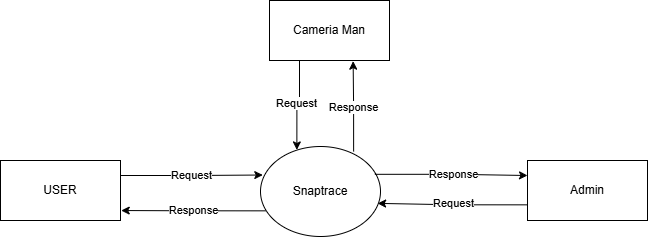
\includegraphics[width=1\textwidth]{dfd/leve0.drawio.png}\par
\vspace{0.5cm}

\noindent \textbf{b). DFD Level 1 Admin}\nopagebreak\par
\vspace{0.2cm}\nopagebreak
\noindent 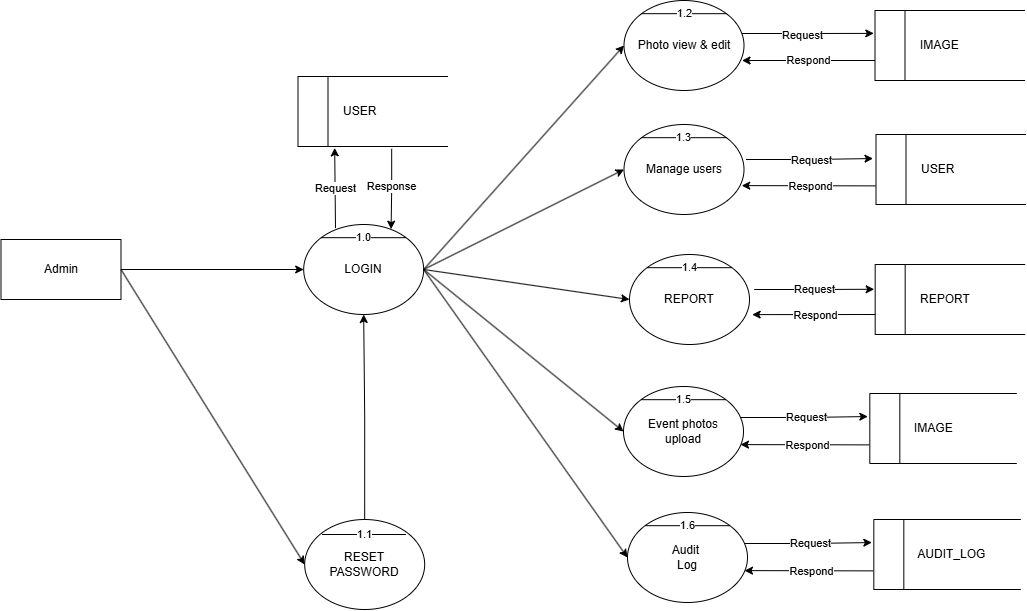
\includegraphics[width=1\textwidth]{dfd/admin.png}\par
\vspace{0.5cm}

\noindent \textbf{c). DFD Level 1 Cameraman}\nopagebreak\par
\vspace{0.2cm}\nopagebreak
\noindent 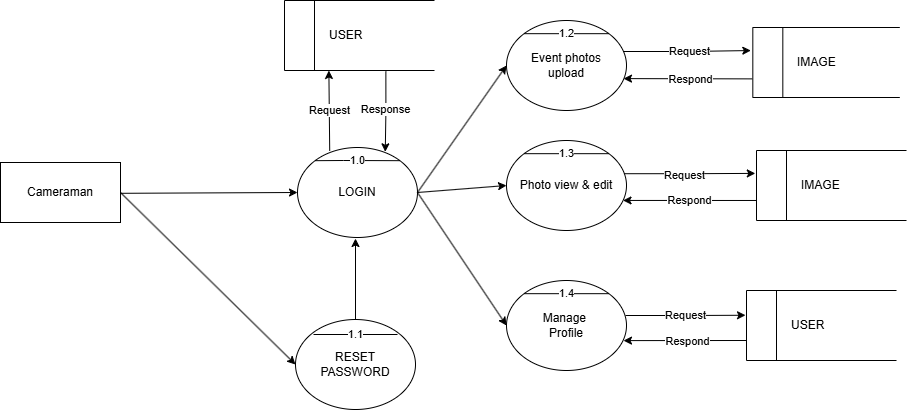
\includegraphics[width=1\textwidth]{dfd/cameraman.png}\par
\vspace{0.5cm}


\noindent \textbf{d). DFD Level 1 User}\nopagebreak\par
\vspace{0.2cm}\nopagebreak
\noindent \includegraphics[width=1\textwidth]{dfd/user.png}\par
\vspace{0.5cm}



\clearpage
\begin{center}
    \vspace*{\fill}
    % \fontsize{Size}{LineSpacing}\selectfont
    % Change 80 to 100 or 120 if you want it even bigger!
    \fontsize{28}{28}\selectfont \textbf{WEB APPLICATION DEVELOPMENT AND DATABASE MANAGEMENT}
    \vspace*{\fill}
\end{center}
\clearpage

\heading{9. WEB APPLICATION DEVELOPMENT AND DATABASE MANAGEMENT}

\subheading{WEB APPLICATION DEVELOPMENT}

\para{Web application development is the process of designing, developing, testing, and maintaining applications that users can access through a web browser over a network. Unlike traditional desktop applications, web applications generally do not require users to install the complete application on their devices. Instead, users can access the application through browsers such as Google Chrome, Mozilla Firefox, and Microsoft Edge.}

\para{SnapTrace is a web-based application developed to simplify the management and distribution of event photographs using facial-recognition technology. It provides different functionalities for registered users, photographers, and administrators. Users can register, submit a reference selfie, and view photographs associated with their accounts. Photographers can upload event photographs for processing, while administrators can access available management and reporting functions.}

\para{Web application development can be divided into two major areas: frontend development and backend development.}

\subheading{Frontend Development}

\para{Frontend development involves creating the user interface through which users interact with the application. It uses technologies such as HTML, CSS, and JavaScript to structure, style, and implement interactive web pages.}

\para{SnapTrace uses React 19 to develop its user interface, Vite 8 as the development and build tool, and React Router DOM 7 for client-side navigation. CSS is used to style the interface, while JavaScript handles application interactions and frontend logic. The frontend communicates with the backend through API requests to perform operations such as authentication, selfie submission, photograph uploads, and gallery retrieval.}

\subheading{Backend Development}

\para{Backend development handles application logic, request processing, authentication, database communication, and other operations that occur on the server. It receives requests from the frontend, processes the submitted information, interacts with the database, and returns appropriate responses.}

\para{SnapTrace uses Node.js as its server-side JavaScript runtime and Express.js to implement REST API endpoints. The backend manages user authentication, role-based authorization, file uploads, image processing, facial recognition, gallery associations, and reporting operations.}

\para{The facial-recognition workflow uses @vladmandic/face-api, TensorFlow.js, and the WebAssembly backend. It detects faces in images, generates numerical facial descriptors, and compares them to identify potentially relevant photographs. The Sharp library is used to resize uploaded images, optimize image files, and generate thumbnails. Photograph matching is performed through an asynchronous in-process queue so that the upload response does not need to wait for the entire matching process to finish.}

\para{Web applications commonly use databases to store persistent information such as user accounts, application settings, uploaded image metadata, and other records. In SnapTrace, the frontend, backend, and database work together to provide a centralized platform for event photograph management.}

\subheading{WHAT IS A DATABASE? WHY IS IT IMPORTANT FOR WEB DEVELOPMENT?}

\para{Data refers to information that can be collected, stored, processed, and retrieved, such as text, numerical values, account information, and image metadata. A database is an organized collection of data that allows efficient storage and retrieval, and a Database Management System (DBMS) is the software used to create, manage, and access it.}

\para{Databases are important in web applications because information such as account details and settings must persist between user sessions and across server restarts. Database systems are commonly classified as relational, document-oriented, key-value, graph, or object-oriented. A relational database organizes data into tables of rows and columns, connected through keys and constraints.}

\para{Structured Query Language (SQL) is used with relational databases to perform CRUD operations: Create, Read, Update, and Delete. Relational systems also support constraints and transactions that help maintain data consistency.}

\para{SnapTrace uses MySQL Community Server 8.0.46 to store user records, settings, image metadata, user--photograph associations, administrative audit records, report metadata, and password-reset tokens. The users table also stores facial descriptors as JSON data for facial matching.}

\para{The database supports authentication and personalized content delivery. After a user logs in, the backend verifies the credentials and uses the authenticated identity to control access to protected operations. When facial matching finds a potential match, the association between the user and the photograph is recorded, and the personalized gallery uses these associations to retrieve the user's photographs.}

\para{Primary keys identify individual records, while foreign keys establish relationships and maintain referential integrity. The user\_gallery\_photos table maps users to images, so one user can be linked to many photographs and one photograph to many users. The Node.js backend accesses MySQL through the mysql2/promise library, and parameterized queries help reduce the risk of SQL injection.}

\para{In conclusion, web development and database management are essential to SnapTrace. React provides the interactive frontend, Node.js and Express.js handle server-side operations, and MySQL maintains persistent data. Together with facial recognition and image processing, they let SnapTrace organize event photographs, match them to registered users, and provide personalized gallery access.}
\clearpage
\begin{center}
    \vspace*{\fill}
    % \fontsize{Size}{LineSpacing}\selectfont
    % Change 80 to 100 or 120 if you want it even bigger!
    \fontsize{28}{28}\selectfont \textbf{TABLES}
    \vspace*{\fill}
\end{center}
\clearpage

\heading{10. TABLES}
% a). Admin Audit Log
\noindent\textbf{a). Admin Audit Log}
\vspace{0.2cm}
\begin{center}
    \renewcommand{\arraystretch}{1.3}
    \begin{tabular}{|>{\raggedright\arraybackslash}p{3.0cm}|>{\raggedright\arraybackslash}p{4.5cm}|>{\raggedright\arraybackslash}p{8.5cm}|}
        \hline
        \rowcolor{lightgray!50}
        \textbf{FIELD} & \textbf{TYPE} & \textbf{CONSTRAINT}                    \\ \hline
        id             & INT UNSIGNED  & PRIMARY KEY, AUTO\_INCREMENT, NOT NULL \\ \hline
        admin\_id      & INT           & NOT NULL (no declared FK in migration) \\ \hline
        action         & VARCHAR(50)   & NOT NULL                               \\ \hline
        target\_type   & VARCHAR(30)   & NOT NULL                               \\ \hline
        target\_id     & INT           & DEFAULT NULL                           \\ \hline
        ip\_address    & VARCHAR(45)   & DEFAULT NULL                           \\ \hline
        user\_agent    & VARCHAR(500)  & DEFAULT NULL                           \\ \hline
        success        & TINYINT(1)    & NOT NULL, DEFAULT 1                    \\ \hline
        metadata       & JSON          & DEFAULT NULL                           \\ \hline
        created\_at    & DATETIME      & NOT NULL, DEFAULT CURRENT\_TIMESTAMP   \\ \hline
    \end{tabular}
\end{center}

\vspace{0.4cm}

% c). Password Token
\noindent\textbf{b). Password Token}
\vspace{0.2cm}
\begin{center}
    \renewcommand{\arraystretch}{1.3}
    \begin{tabular}{|>{\raggedright\arraybackslash}p{3.0cm}|>{\raggedright\arraybackslash}p{4.5cm}|>{\raggedright\arraybackslash}p{8.5cm}|}
        \hline
        \rowcolor{lightgray!50}
        \textbf{FIELD} & \textbf{TYPE} & \textbf{CONSTRAINT}                                                                              \\ \hline
        id             & INT UNSIGNED  & PRIMARY KEY, AUTO\_INCREMENT, NOT NULL                                                           \\ \hline
        user\_id       & INT UNSIGNED  & NOT NULL, FOREIGN KEY $\rightarrow$ users.id, ON DELETE CASCADE (signedness mismatch documented) \\ \hline
        token          & VARCHAR(255)  & UNIQUE, NOT NULL                                                                                 \\ \hline
        expires\_at    & DATETIME      & NOT NULL                                                                                         \\ \hline
        used           & TINYINT(1)    & NOT NULL, DEFAULT 0                                                                              \\ \hline
        created\_at    & DATETIME      & NOT NULL, DEFAULT CURRENT\_TIMESTAMP                                                             \\ \hline
    \end{tabular}
\end{center}

\clearpage
% b). Image
\noindent\textbf{c). Image}
\vspace{0.2cm}
\begin{center}
    \renewcommand{\arraystretch}{1.3}
    \begin{tabular}{|>{\raggedright\arraybackslash}p{3.0cm}|>{\raggedright\arraybackslash}p{4.5cm}|>{\raggedright\arraybackslash}p{8.5cm}|}
        \hline
        \rowcolor{lightgray!50}
        \textbf{FIELD}  & \textbf{TYPE}                                        & \textbf{CONSTRAINT}                    \\ \hline
        id              & INT                                                  & PRIMARY KEY, AUTO\_INCREMENT, NOT NULL \\ \hline
        filename        & VARCHAR(255)                                         & NOT NULL                               \\ \hline
        filepath        & VARCHAR(500)                                         & NOT NULL                               \\ \hline
        original\_name  & VARCHAR(255)                                         & DEFAULT NULL                           \\ \hline
        mime\_type      & VARCHAR(100)                                         & DEFAULT NULL                           \\ \hline
        file\_size      & BIGINT UNSIGNED                                      & DEFAULT 0                              \\ \hline
        uploaded\_by    & INT                                                  & DEFAULT NULL                           \\ \hline
        uploaded\_at    & TIMESTAMP                                            & DEFAULT CURRENT\_TIMESTAMP             \\ \hline
        thumbnail\_path & VARCHAR(500)                                         & NOT NULL, DEFAULT ''                   \\ \hline
        status          & ENUM('pending', 'processing', 'completed', 'failed') & NOT NULL, DEFAULT 'completed'          \\ \hline
    \end{tabular}
\end{center}

% e). User Gallery
\vspace{0.2cm}
\noindent\textbf{d). User Gallery}
\vspace{0.2cm}
\begin{center}
    \renewcommand{\arraystretch}{1.3}
    \begin{tabular}{|>{\raggedright\arraybackslash}p{3.0cm}|>{\raggedright\arraybackslash}p{4.5cm}|>{\raggedright\arraybackslash}p{8.5cm}|}
        \hline
        \rowcolor{lightgray!50}
        \textbf{FIELD}    & \textbf{TYPE} & \textbf{CONSTRAINT}                                              \\ \hline
        id                & INT           & PRIMARY KEY, AUTO\_INCREMENT, NOT NULL                           \\ \hline
        user\_id          & INT           & NOT NULL, FOREIGN KEY $\rightarrow$ users.id, ON DELETE CASCADE  \\ \hline
        photo\_id         & INT           & NOT NULL, FOREIGN KEY $\rightarrow$ images.id, ON DELETE CASCADE \\ \hline
        match\_confidence & FLOAT         & NOT NULL, DEFAULT 0                                              \\ \hline
        matched\_at       & DATETIME      & NOT NULL, DEFAULT CURRENT\_TIMESTAMP                             \\ \hline
    \end{tabular}
\end{center}


\clearpage
% d). Reports
\noindent\textbf{e). Reports}
\vspace{0.2cm}
\begin{center}
    \renewcommand{\arraystretch}{1.3}
    \begin{tabular}{|>{\raggedright\arraybackslash}p{3.0cm}|>{\raggedright\arraybackslash}p{4.5cm}|>{\raggedright\arraybackslash}p{8.5cm}|}
        \hline
        \rowcolor{lightgray!50}
        \textbf{FIELD} & \textbf{TYPE}                                       & \textbf{CONSTRAINT}                    \\ \hline
        id             & INT UNSIGNED                                        & PRIMARY KEY, AUTO\_INCREMENT, NOT NULL \\ \hline
        name           & VARCHAR(255)                                        & NOT NULL                               \\ \hline
        type           & VARCHAR(50)                                         & NOT NULL                               \\ \hline
        status         & ENUM('queued', 'generating', 'completed', 'failed') & NOT NULL, DEFAULT 'queued'             \\ \hline
        generated\_by  & INT                                                 & NOT NULL (no declared FK in migration) \\ \hline
        file\_path     & VARCHAR(500)                                        & DEFAULT NULL                           \\ \hline
        metadata       & JSON                                                & DEFAULT NULL                           \\ \hline
        created\_at    & DATETIME                                            & NOT NULL, DEFAULT CURRENT\_TIMESTAMP   \\ \hline
        completed\_at  & DATETIME                                            & DEFAULT NULL                           \\ \hline
    \end{tabular}
\end{center}

\vspace{0.4cm}
% f). User Settings
\noindent\textbf{f). User Settings}
\vspace{0.2cm}
\begin{center}
    \renewcommand{\arraystretch}{1.3}
    \begin{tabular}{|>{\raggedright\arraybackslash}p{3.0cm}|>{\raggedright\arraybackslash}p{4.5cm}|>{\raggedright\arraybackslash}p{8.5cm}|}
        \hline
        \rowcolor{lightgray!50}
        \textbf{FIELD} & \textbf{TYPE} & \textbf{CONSTRAINT}                                                \\ \hline
        user\_id       & INT           & PRIMARY KEY, FOREIGN KEY $\rightarrow$ users.id, ON DELETE CASCADE \\ \hline
        viewed\_photos & TINYINT(1)    & NOT NULL, DEFAULT 1                                                \\ \hline
        email\_photos  & TINYINT(1)    & NOT NULL, DEFAULT 1                                                \\ \hline
        keep\_face     & TINYINT(1)    & NOT NULL, DEFAULT 0                                                \\ \hline
        email\_notifs  & TINYINT(1)    & NOT NULL, DEFAULT 1                                                \\ \hline
        sms\_notifs    & TINYINT(1)    & NOT NULL, DEFAULT 0                                                \\ \hline
        marketing      & TINYINT(1)    & NOT NULL, DEFAULT 0                                                \\ \hline
    \end{tabular}
\end{center}

\vspace{0.4cm}
\clearpage
% g). User
\noindent\textbf{g). User}
\vspace{0.2cm}
\begin{center}
    \renewcommand{\arraystretch}{1.3}
    \begin{tabular}{|>{\raggedright\arraybackslash}p{3.0cm}|>{\raggedright\arraybackslash}p{4.5cm}|>{\raggedright\arraybackslash}p{8.5cm}|}
        \hline
        \rowcolor{lightgray!50}
        \textbf{FIELD}      & \textbf{TYPE}                           & \textbf{CONSTRAINT}                                      \\ \hline
        id                  & INT                                     & PRIMARY KEY, AUTO\_INCREMENT, NOT NULL                   \\ \hline
        first\_name         & VARCHAR(100)                            & NOT NULL                                                 \\ \hline
        last\_name          & VARCHAR(100)                            & NOT NULL                                                 \\ \hline
        email               & VARCHAR(255)                            & UNIQUE, NOT NULL                                         \\ \hline
        password            & VARCHAR(255)                            & NOT NULL                                                 \\ \hline
        role                & VARCHAR(20)                             & NOT NULL, DEFAULT 'user'                                 \\ \hline
        status              & ENUM('active', 'suspended', 'inactive') & NOT NULL, DEFAULT 'active'                               \\ \hline
        token\_valid\_after & DATETIME                                & DEFAULT NULL                                             \\ \hline
        created\_at         & TIMESTAMP                               & DEFAULT CURRENT\_TIMESTAMP                               \\ \hline
        last\_login\_at     & DATETIME                                & DEFAULT NULL                                             \\ \hline
        updated\_at         & DATETIME                                & DEFAULT CURRENT\_TIMESTAMP, ON UPDATE CURRENT\_TIMESTAMP \\ \hline
        phone               & VARCHAR(30)                             & DEFAULT NULL                                             \\ \hline
        avatar\_url         & VARCHAR(500)                            & DEFAULT NULL                                             \\ \hline
        face\_scan\_url     & VARCHAR(500)                            & DEFAULT NULL                                             \\ \hline
    \end{tabular}
\end{center}

\clearpage

\begin{center}
    \vspace*{\fill}
    % \fontsize{Size}{LineSpacing}\selectfont
    % Change 80 to 100 or 120 if you want it even bigger!
    \fontsize{28}{28}\selectfont \textbf{SYSTEM TESTING}
    \vspace*{\fill}
\end{center}
\clearpage

\heading{11. SYSTEM TESTING}

\para{System testing is an important phase of software development and quality assurance. It involves evaluating the behaviour of a software application to determine whether it satisfies the specified requirements. Testing helps identify errors, verify the correctness of individual modules, and examine the interaction between different components of the system.}

\para{SnapTrace is an Intelligent Event Media Management and Biometric Distribution System developed to simplify the identification and distribution of event photographs using facial-recognition technology. Testing of SnapTrace focuses on user authentication, reference selfie enrollment, event photograph uploads, image processing, facial matching, personalized galleries, database operations, and administrative functions.}

\para{The backend application uses Vitest for automated testing. The recorded test execution includes five backend test suites containing 44 tests, all of which passed. However, these results represent only the behaviours covered by those tests. Comprehensive frontend end-to-end testing, formal user acceptance testing, performance benchmarking, and biometric accuracy evaluation have not been established by the available test evidence.}

\subheading{11.1 TESTING TECHNIQUES}

\para{Software testing can be performed at different levels to evaluate the correctness and reliability of an application. The following testing techniques are relevant to SnapTrace:}

\begin{itemize}
    \item Unit Testing
    \item Integration Testing
    \item Validation Testing
    \item System Testing
    \item Output Testing
    \item User Acceptance Testing
\end{itemize}

\para{Each technique focuses on a different aspect of the application. The following sections describe how these techniques apply to SnapTrace and distinguish verified results from testing activities that require further execution.}
\clearpage
\subheading{11.1.1 UNIT TESTING}

\para{Unit testing is the process of testing individual functions, components, or modules to verify that they produce the expected results. It is generally performed during development to identify errors before the modules are integrated into the complete application.}

\para{SnapTrace uses Vitest as its backend testing framework. Automated tests are used to verify selected backend operations and application logic. The reported test execution contains five backend test suites with 44 tests.}

\subheading{Recorded Test Result:}

\begin{itemize}
    \item Testing framework: Vitest
    \item Number of test suites: 5
    \item Total tests: 44
    \item Passed tests: 44
    \item Failed tests: 0
\end{itemize}

\para{The results indicate that all 44 tests passed during the recorded execution. This provides evidence that the behaviours covered by those tests worked as expected in that run. However, it does not establish complete test coverage of every module. The facial-recognition inference pipeline and asynchronous image-processing queue are not comprehensively covered by the available unit-test evidence.}

\subheading{11.1.2 INTEGRATION TESTING}

\para{Integration testing examines whether different modules communicate correctly and exchange information as expected. It focuses on identifying problems at the interfaces between application components.}

\para{SnapTrace integrates a React frontend with a Node.js and Express backend through REST API endpoints. The backend communicates with the MySQL database using the mysql2/promise library. It also integrates file-upload handling, image processing, facial-recognition services, and gallery-management operations.}

\para{Integration testing should verify the following interactions:}

\begin{itemize}
    \item Communication between the frontend and backend API.
    \item Database insertion, retrieval, and updating of application records.
    \item Uploading and storing reference selfies and event photographs.
    \item Processing photographs and generating facial descriptors.
    \item Creating associations between users and potentially matching photographs.
    \item Retrieving the correct photographs for a user's personalized gallery.
\end{itemize}

\para{These checks are important for ensuring that individual modules work together correctly. Comprehensive integration-test completion has not been established by the available test results; therefore, the above activities should be recorded as completed only after they have been executed and their results documented.}

\subheading{11.1.3 VALIDATION TESTING}

\para{Validation testing determines whether the software meets its intended functional requirements. It examines whether the system accepts valid inputs, rejects invalid inputs, and performs the operations expected by its users.}

\para{SnapTrace includes validation rules for reference selfies and event photograph uploads. Reference selfies must be in JPEG or PNG format and must not exceed 5 MB. The enrollment workflow requires exactly one detected face. Event photograph uploads accept JPEG or PNG files, with a maximum file size of 30 MB per file and a maximum of 10 files per request.}

\para{Validation testing should include the following cases:}

\begin{itemize}
    \item Submitting valid registration and login information.
    \item Uploading a reference selfie in a supported format.
    \item Attempting to upload a selfie exceeding the configured file-size limit.
    \item Submitting a selfie containing no detectable face or multiple faces.
    \item Uploading an unsupported image format.
    \item Attempting to upload event photographs exceeding the configured file-size or file-count limits.
    \item Submitting invalid credentials or unauthorized requests.
\end{itemize}

\para{The implementation of these validation rules does not, by itself, demonstrate that every case has been tested successfully. Actual results should be recorded after executing the relevant test cases.}

\subheading{11.1.4 SYSTEM TESTING}

\para{System testing evaluates the application as a complete system. It examines whether the frontend, backend, database, authentication mechanisms, image-processing operations, and facial-recognition workflow function together as intended.}

\para{For SnapTrace, system testing should cover the complete workflow:}

\begin{itemize}
    \item 1. A user registers and logs in to the application.
    \item 2. The user submits a reference selfie for facial enrollment.
    \item 3. A photographer uploads event photographs.
    \item 4. The backend accepts the uploaded photographs and initiates background processing.
    \item 5. The facial-recognition pipeline detects faces and compares their descriptors with registered user descriptors.
    \item 6. Potential matches are associated with the relevant users.
    \item 7. Users access their personalized galleries.
    \item 8. Authorized administrators access the available management and reporting functions.
\end{itemize}

\para{The system uses an Euclidean-distance threshold of 0.50 or lower to identify potential facial matches. This is a configured matching criterion and is not a measured accuracy percentage.}

\para{System testing should also examine error handling, authorization restrictions, database consistency, and the handling of uploaded media. Although the backend unit tests have passed, comprehensive end-to-end system testing has not been established by the available evidence.}

\subheading{11.1.5 OUTPUT TESTING}

\para{Output testing verifies whether the information generated by an application is correct, accessible, and presented in the expected format. It examines the results produced by different application operations.}

\para{SnapTrace generates several types of output, including authentication responses, photograph upload responses, personalized galleries, processed images, thumbnails, administrative information, and JSON reports.}

\para{Output testing should verify the following:}

\begin{itemize}
    \item Successful authentication produces the expected response.
    \item Invalid authentication attempts are rejected appropriately.
    \item Accepted photograph uploads return the expected HTTP response.
    \item Processed photographs and thumbnails can be retrieved and displayed correctly.
    \item Personalized galleries display photographs associated with the appropriate user.
    \item JSON reports are generated in the expected format.
    \item Report metadata is stored correctly in the database.
    \item Errors are communicated through appropriate responses.
\end{itemize}

\para{In SnapTrace, an HTTP 201 response indicates that the upload request has been accepted and processed according to the upload operation. It does not necessarily mean that background facial matching has finished. Output testing must therefore distinguish between successful upload acceptance and completion of the matching workflow.}

\para{Comprehensive output-test results have not been established by the available evidence and should be documented after the relevant checks are performed.}
\clearpage
\subheading{11.1.6 USER ACCEPTANCE TESTING}

\para{User Acceptance Testing (UAT) evaluates whether the system meets the practical requirements and expectations of its intended users. It typically involves representative users performing common tasks and reviewing whether the application supports their needs.}

\para{For SnapTrace, the intended user groups include registered users, photographers, and administrators. Acceptance testing can be conducted using representative scenarios such as:}

\begin{itemize}
    \item Registering an account and logging in.
    \item Submitting a reference selfie.
    \item Uploading event photographs.
    \item Checking whether matching photographs appear in a personalized gallery.
    \item Reviewing available administrative functions.
    \item Generating and accessing reports.
    \item Evaluating the clarity of error messages and the ease of navigating the application.
\end{itemize}

\para{During UAT, the tester should record the test scenario, expected result, actual result, status, and any issues encountered. Feedback should be used to identify usability problems and areas requiring improvement.}

\para{Formal user acceptance testing with documented results has not been established in the available project information. Therefore, these scenarios are presented as a proposed acceptance-testing procedure rather than completed UAT.}

\subheading{11.1.7 TESTING SUMMARY}

\para{The SnapTrace project includes automated backend testing using Vitest. The recorded execution contains five test suites and 44 tests, all of which passed. This demonstrates successful execution of the behaviours covered by those tests.}

\para{The current test evidence does not establish that all modules and workflows have been comprehensively tested. Further verification is required for integration between application components, the complete facial-recognition workflow, asynchronous image processing, frontend interactions, and end-to-end gallery distribution.}

\para{Performance testing, formal security assessment, user acceptance testing, and biometric accuracy benchmarking also require separate evaluation before the application can be considered fully verified for production deployment.}

\para{Overall, the completed backend unit tests provide a foundation for software quality assurance. Additional testing and documented results will strengthen confidence in SnapTrace's functional correctness, reliability, security, and suitability for real-world event media management.}

\clearpage
\begin{center}
    \vspace*{\fill}
    % \fontsize{Size}{LineSpacing}\selectfont
    % Change 80 to 100 or 120 if you want it even bigger!
    \fontsize{28}{28}\selectfont \textbf{NORMALIZATION}
    \vspace*{\fill}
\end{center}
\clearpage

\heading{12. NORMALIZATION}

\para{Database normalization is the process of organizing data into tables to reduce unnecessary duplication and improve data consistency. It involves dividing data into related tables and establishing relationships between them using primary keys and foreign keys. Normalization helps minimize data redundancy, prevent insertion, update, and deletion anomalies, and maintain the integrity of stored information.}

\para{In SnapTrace, MySQL is used to manage user accounts, user settings, uploaded image information, personalized gallery associations, administrative audit records, reports, and password-reset tokens. The database contains seven principal tables: users, user\_settings, images, user\_gallery\_photos, admin\_audit\_log, reports, and password\_reset\_tokens.}

\para{The database structure uses primary keys to identify records and relationships to connect related information. The following normal forms provide a basis for understanding the organization of the SnapTrace database.}

\para{The normal forms considered are:}

\begin{itemize}
    \item First Normal Form (1NF)
    \item Second Normal Form (2NF)
    \item Third Normal Form (3NF)
\end{itemize}

\subheading{12.1 FIRST NORMAL FORM (1NF)}

\para{A relation is in First Normal Form when each field contains a single value from its defined domain, each row can be uniquely identified, and repeating groups or multivalued attributes are not stored as repeated columns.}

\para{In SnapTrace, the database uses individual records to store user accounts, images, user settings, gallery associations, reports, audit activities, and password-reset tokens. Primary keys identify individual records in the tables.}

\para{For example, the users table stores account information, while the images table stores information about uploaded photographs. The user\_gallery\_photos table stores individual associations between users and matched images instead of storing a list of image associations in a single relational field.}

\para{The face\_embedding column in the users table stores a facial descriptor as JSON data. Although JSON is used to represent the descriptor, this does not automatically establish that the entire table satisfies every 1NF requirement. Formal verification depends on the intended relational model and how the field is treated.}

\clearpage

\subheading{12.2 SECOND NORMAL FORM (2NF)}

\para{A relation is in Second Normal Form when it satisfies First Normal Form and every non-key attribute depends on the whole candidate key rather than only part of a composite candidate key. This condition is especially important for tables that use composite keys.}

\para{In SnapTrace, the user\_gallery\_photos table associates users with images and includes attributes such as match\_confidence and matched\_at. The combination of user\_id and photo\_id is subject to a unique constraint, preventing duplicate associations for the same user and image.}

\para{The attributes describing a particular gallery association belong to that association rather than independently to the user or image. The users and images tables separately store user-related and image-related information.}

\para{This structure helps avoid unnecessary duplication of user and image details within the gallery association table. A complete determination of 2NF status would require checking the candidate keys and functional dependencies of every table.}
\subheading{12.3 THIRD NORMAL FORM (3NF)}

\para{A relation is in Third Normal Form when it satisfies Second Normal Form and its non-key attributes do not have inappropriate transitive dependencies on a candidate key. In practical terms, non-key attributes should describe the entity represented by the table rather than depend on other non-key attributes.}

\para{SnapTrace separates information according to its purpose. The users table stores account-related information, user\_settings stores user preferences, and images stores uploaded-image information. The user\_gallery\_photos table records the relationship between a user and an image. Similarly, password\_reset\_tokens stores password-reset information, admin\_audit\_log records administrative activities, and reports maintains report-related metadata.}

\para{This separation supports organized data storage and reduces the need to repeat the same information across multiple tables. Relationships between tables allow the application to retrieve associated data when required.}

\para{However, the actual normalization status of the entire database cannot be confirmed solely from the table names and descriptions. It requires examining the complete column definitions, candidate keys, and functional dependencies. Therefore, the SnapTrace database is designed using relational separation and relationships that support normalization, but universal compliance with 3NF should only be claimed after a formal schema review.}
\clearpage
\begin{center}
    \vspace*{\fill}
    % \fontsize{Size}{LineSpacing}\selectfont
    % Change 80 to 100 or 120 if you want it even bigger!
    \fontsize{28}{28}\selectfont \textbf{FUTURE ENHANCEMENT}
    \vspace*{\fill}
\end{center}
\clearpage
\heading{13. FUTURE ENHANCEMENT}

\para{SnapTrace offers several opportunities for future enhancement in functionality, scalability, security, and user experience. A dedicated mobile application or Progressive Web Application (PWA) would let users and photographers access the system conveniently from smartphones and tablets, simplifying selfie submission, photograph browsing, and gallery access. Cloud-based object storage would help manage large photograph collections as the number of users and images grows, and a durable background-processing system using tools such as Redis and BullMQ would make photograph-processing jobs more reliable during large events or server restarts.}

\para{The facial-recognition module could be improved through systematic accuracy evaluation using representative datasets and documented performance metrics. Further work could include optimizing image-processing workflows, handling low-quality photographs better, and evaluating alternative face-matching methods. Any change to the matching algorithm should be validated before deployment to ensure it improves performance without introducing unacceptable matching errors. For larger deployments, vector indexing technologies such as FAISS or Milvus could be evaluated to speed up facial-descriptor searches across large user collections.}

\para{Security and privacy could be strengthened by storing password-reset tokens as cryptographic hashes, restricting direct access to uploaded media, and improving the management of signing secrets. Additional measures include multi-factor authentication, configurable data-retention policies, automated deletion of expired data, and clearer consent and privacy-management workflows, supporting more responsible handling of reference selfies, facial descriptors, and event photographs.}

\para{The user experience and administration could be enhanced with real-time processing-status indicators and notifications, along with a more advanced administrative dashboard showing statistics on uploads, processing failures, gallery associations, and system usage. Multi-language support could also make the application more accessible to users from different linguistic backgrounds.}

\para{Finally, comprehensive frontend and end-to-end automated testing, load testing, security assessment, and usability evaluation with representative users would provide stronger evidence of reliability and production readiness. By introducing these enhancements incrementally, SnapTrace could evolve into a more scalable, secure, and efficient platform for managing and distributing event photographs.}
\clearpage
\begin{center}
    \vspace*{\fill}
    % \fontsize{Size}{LineSpacing}\selectfont
    % Change 80 to 100 or 120 if you want it even bigger!
    \fontsize{28}{28}\selectfont \textbf{CONCLUSION}
    \vspace*{\fill}
\end{center}
\clearpage
\heading{14. CONCLUSION}

\para{The {\bfseries{SnapTrace}} project provides an intelligent and user-friendly solution for managing event photographs using facial recognition technology. The system addresses the common difficulty of finding individual photographs among large collections of event images by enabling users to access photographs that match their registered facial images. It simplifies the process of organizing, searching, and retrieving event photographs through a centralized web-based platform.}
\para{The system integrates modern web technologies, including {\bfseries{React, Vite, Node.js, Express.js, and MySQL}}, to support user authentication, reference selfie registration, event photo uploads, facial recognition-based matching, personalized photo galleries, and administrative management. It also provides features for photographers to upload event photographs and for administrators to manage users, monitor system activities, and generate reports. These functionalities demonstrate the practical application of web development, database management, and facial recognition concepts in solving a real-world problem.}
\para{The development of SnapTrace demonstrates how automation and biometric image processing can improve the accessibility and organization of digital photographs. The system establishes a foundation for simplifying photo discovery and reducing the need for manual searching. However, the effectiveness of facial matching depends on factors such as image quality, lighting conditions, facial visibility, and the reliability of the recognition process. Appropriate attention to authentication, data protection, and the handling of facial information is also essential for responsible system operation.}
\para{In conclusion, {\bfseries{SnapTrace represents a practical application of intelligent image management and facial recognition in event photography}}. The project provides a foundation for future enhancements, including improved recognition performance, more efficient processing of large photo collections, enhanced privacy controls, and expanded reporting capabilities. With further testing and development, SnapTrace can evolve into a more comprehensive platform for managing and retrieving event photographs efficiently.}
\clearpage
\begin{center}
    \vspace*{\fill}
    % \fontsize{Size}{LineSpacing}\selectfont
    % Change 80 to 100 or 120 if you want it even bigger!
    \fontsize{28}{28}\selectfont \textbf{REFERENCES}
    \vspace*{\fill}
\end{center}
\clearpage

\heading{15. REFERENCES}

\begin{enumerate}
    \item React Documentation. \textit{React – The Library for Web and Native User Interfaces.} Available at: \url{https://react.dev/}

    \item Vite Documentation. \textit{Vite – Next Generation Frontend Tooling.} Available at: \url{https://vite.dev/}

    \item Node.js Documentation. \textit{Node.js – JavaScript Runtime Environment.} Available at: \url{https://nodejs.org/docs/}

    \item Express.js Documentation. \textit{Express – Node.js Web Application Framework.} Available at: \url{https://expressjs.com/}

    \item MySQL Documentation. \textit{MySQL Reference Manual.} Available at: \url{https://dev.mysql.com/doc/}

    \item OpenCV Documentation. \textit{OpenCV – Open Source Computer Vision Library.} Available at: \url{https://docs.opencv.org/}

    \item MDN Web Docs. \textit{HTML, CSS, and JavaScript Web Development Documentation.} Available at: \url{https://developer.mozilla.org/}

    \item OWASP Foundation. \textit{OWASP Top 10: Web Application Security Risks.} Available at: \url{https://owasp.org/www-project-top-ten/}

    \item Schroff, F., Kalenichenko, D., and Philbin, J. (2015). \textit{FaceNet: A Unified Embedding for Face Recognition and Clustering.} Proceedings of the IEEE Conference on Computer Vision and Pattern Recognition (CVPR), pp. 815–823. \url{https://doi.org/10.1109/CVPR.2015.7298682}

    \item Szeliski, R. (2022). \textit{Computer Vision: Algorithms and Applications.} 2nd edition. Springer. Available at: \url{https://szeliski.org/Book/}
\end{enumerate}

\clearpage
\begin{center}
    \vspace*{\fill}
    % \fontsize{Size}{LineSpacing}\selectfont
    % Change 80 to 100 or 120 if you want it even bigger!
    \fontsize{28}{28}\selectfont \textbf{APPENDIX}
    \vspace*{\fill}
\end{center}
\clearpage
